\chapter{Dostupné platformy}

Pro \legoEV{} existuje mnoho vývojových platforem. 
Většinou se jedná o~specificky navržené programovací API ve~spojení s~vývojovým prostředím. 
Tyto platformy většinou využívají oficiální systém v~\EVthree{}, ale jsou i~platformy s~vlastním operačním systémem. 
V~tomto textu bude popsán jen výběr těch nejzajímavějších. % platforem. 

\section{Originální prostředí od \lego}

V rámci této podkapitoly bude rozebrán samotný operační systém na \EVthree{} a také vývojové prostředí určené pro tvorbu a ladění programů. 
\lego{} si pro \EVthree{} vytvořilo vlastní operační systém postavený na linuxovém jádru \cite{legoMindstormsEV3_fw-dev-kit}. 
Uvnitř systému běží virtuální stroj, který zpracovává byte-code uživatelské aplikace. 
Byte-code je vytvořen ve~vývojovém prostředí na PC a~odeslán do \brick{\it u}. 

Celý systém s~vývojářskými nástroji a~dokumentací je volně k~dispozici na~webu \lego{}~\cite{legoMindstorms_download}. Díky tomu, že~\lego{} uvolnilo zdrojové kódy, mohly vzniknout alternativní systémy pro~\EVthree{} jako~\evThreeDev{} nebo \evRT. 

\subsection{\legoSW{}}
\begin{figure}[h]
	\centering
	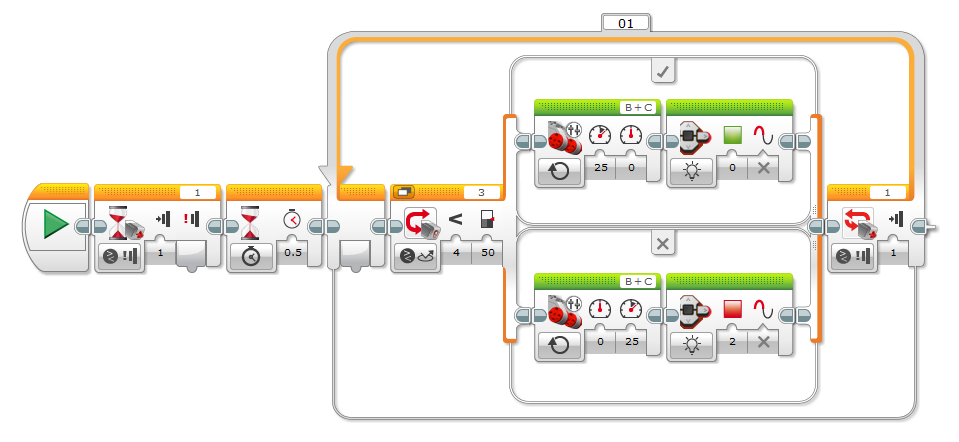
\includegraphics[width=0.99\textwidth]{images/lego-soft/lego-soft_robotut_switch-touch+motors+leds.png}
	\caption{Ukázka programovacích bloků v \legoSW}
	\label{fig:lego-soft_example-blocks}
\end{figure}

% * <kuba.streit@gmail.com> 2017-05-07T14:22:57.674Z:
% 
% Nebyl by lepší například program line_simple z RoboWeekendu? Je tam navíc podmínka. Tady jsou jen 2 cykly.
% 
% ^ <paral.jarek@gmail.com> 2017-05-07T19:09:07.729Z:
%
% JJ byl. Jen přemýšlím, jestli na začátek ještě nepřidat waitForPressBtn. Co myslíš?
%
% ^ <paral.jarek@gmail.com> 2017-05-07T20:00:24.693Z:
%
% Obrázek upraven.
%
% ^.
\legoSW{} je~vývojářský program, který je k~\EVthree{} dostupný zdarma. 
Tento  software vytvořilo \lego{} ve~spolupráci s~firmou \NI{}. 
Je~tudíž postavený na~vývojovém prostředí \labview{}. 
\lego{} s~\NI{} již~spolupracovalo na předešlých vývojových prostředích. % pro~\legoM{}. %  a~proto ani tentokrát neudělalo výjimku.  
Program se~snaží působit jako profesionální vývojové a~laboratorní studio, což se~mu celkem daří.
Nabízí celou řadu funkcí od modulu pro programování, přes tvorbu různých experimentů až~po přípravy interaktivních návodů a~průvodců programováním v~tomto prostředí.



V~režimu tvorby programu jsou hlavními stavebními kameny \EVblocks, které se ve~formě diagramů skládají do podoby výsledného programu (obrázek \ref{fig:lego-soft_example-blocks}).
Bloky jsou rozděleny do~několika skupin (akční, tok programu, senzory, datové operace, pokročilé a~vlastní), které se liší svojí barvou a použitím. 
Pomocí těchto bloků lze řídit tok programu (podmínky, cykly, čekání a vlákna), pracovat s~proměnnými, obsluhovat senzory, provádět matematické operace a~nebo i~využívat vlastní bloky.

\begin{figure}[h]
	\centering
	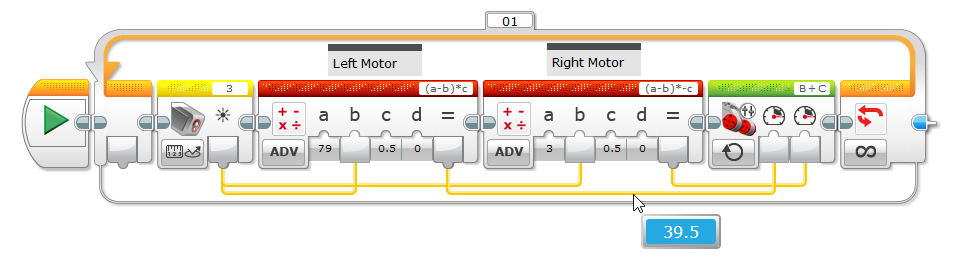
\includegraphics[width=\textwidth]{images/lego-soft/lego-soft_live-debuging_line-advance.png}
	\caption{Ukázka debugování za běhu programu}
	\label{fig:lego-soft_live-debuging_line-advance}
\end{figure}

Vše je pěkně graficky zpracováno a~působí to~jako jednotný celek. 
% * <paral.jarek@gmail.com> 2017-05-07T20:07:55.305Z:
% 
% > jako jednotný celek
% Není tato fráze divná?
% 
% ^.
Při běhu programu lze~sledovat jeho tok (kde v diagramu se program nachází) a~nebo si třeba zobrazit aktuální stav (hodnotu proměnné, výsledek matematické operace, vstupní data ze~senzoru, \dots). 
% * <kuba.streit@gmail.com> 2017-05-07T14:29:43.374Z:
% 
% Z hlediska toho senzoru to jsou výstupní data, ale z hlediska aplikace naopak vstupní. Myslí, že tady se díváš z pohledu aplikace.
% 
% ^ <paral.jarek@gmail.com> 2017-05-07T19:09:35.360Z:
% 
% Souhlas. Upraveno.
% 
% ^.
Ukázku si~lze prohlédnout na obrázku \ref{fig:lego-soft_live-debuging_line-advance}, kde je vidět hodnota 39.5, odpovídající výsledku výpočtu výkonu pro levý motor v~závislosti na~naměřené hodnotě od barevného senzoru.
Zároveň je podle šrafování vrchní lišty bloků vidět, že~program aktuálně probíhá v~daném cyklu.

Pro práci s~\brick{\it em} je k~dispozici modul {\it Správa hardwaru}, kde si lze zjisti informace jako jméno, stav baterie, verze firmwaru nebo obsazenost paměti. 
Umožňuje také jednoduše nahrávat, spouštět a ukončovat programy. 

Je zde i~správa připojení, v~rámci které lze vyhledávat a~připojovat se k dostupným \brick{\it ům}. 
% * <kuba.streit@gmail.com> 2017-05-07T14:32:43.825Z:
% 
% Nebylo by lepší k dostupným brickům (i když tím skloňováním si nejsem úplně jistý).
% 
% ^ <paral.jarek@gmail.com> 2017-05-07T18:55:45.334Z:
% 
% " a~připojovat se k dostupným"
% Uvažoval jsem o tom, ale bylo by to čtvrté Brick v jednom odstavci, Není to moc?
% 
% ^ <paral.jarek@gmail.com> 2017-05-07T20:15:33.294Z:
%
% Co třeba "k dostupným robotům"?
%
% ^ <paral.jarek@gmail.com> 2017-05-07T22:11:21.861Z:
%
% Vyřešeno
%
% ^.
K dispozici jsou tři druhý připojení: USB kabel, Bluetooth a WiFi. Bluetooth je již integrován, ale pro použití WiFi je potřeba připojit WiFi modul.

\begin{figure}[h]
	\begin{minipage}[b]{.48\textwidth}
		\centering
		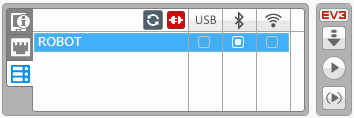
\includegraphics[width=\textwidth]{images/lego-soft/lego-soft_brick-manager_connected.png}
		\caption{Správa připojení k \brick{\it u}}
		\label{fig:lego-soft_brick-manager-connected}
	\end{minipage}
	\hfill
	\begin{minipage}[b]{.48\textwidth}
		\centering
		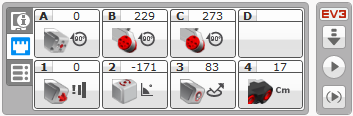
\includegraphics[width=\textwidth]{images/lego-soft/lego-soft_brick_port-view.png}
		\caption{Informační panel s porty}
		\label{fig:lego-soft_brick_port-view}
	\end{minipage}
\end{figure}
Nejzajímavějším panelem je správce portů. 
Zobrazuje na jakém portu je připojen který senzor nebo motor. 
Uživatel může vidět také aktuální hodnoty komponentů a přepínat i jejich režimy.    
Například u barevného senzoru si může vybrat, zda se bude zobrazovat barva nebo odrazivost povrchu. U motorů lze naopak nastavit, jestli má být ujetá vzdálenost zobrazování v otáčkách nebo ve stupních. 
Tento panel považuji ze jednu z nejpodstatnějších funkcí celého programu, jelikož dává uživateli dobrý přehled o aktuálním stavu hardwaru. 
Jednoduše lze tak ladit konstanty v programech (threshold pro barevný senzor při detekci čáry, počet stupňů k dojetí na pozici nebo vzdálenost od překážky měřenou ultrazvukem).
% * <paral.jarek@gmail.com> 2017-05-07T20:26:27.471Z:
% 
% > v otáčkách nebo ve stupních. 
% Je to takhle srozumitelné?
% 
% ^.
\\

Nevýhody \legoSW:
\renewcommand{\labelitemi}{$-$}
\begin{itemize}[noitemsep]\itemsep2pt
	\item náročný na hardware počítače
	\item větší programy se stávají nepřehledné a špatně se v nich orientuje a hledají chyby
	\item nelze editovat proměnné ani rozhraní uživatelských bloků (jejich parametry)
	% * <kuba.streit@gmail.com> 2017-05-07T14:34:04.289Z:
	% 
	% Nelze editovat rozhraní uživatelských bloků. Jejich "kód" editovat můžeš.
	% 
	% ^ <paral.jarek@gmail.com> 2017-05-07T14:53:32.717Z:
	%
	% Jj to máš opravdu. Upraveno.
	%
	% ^.
	\item debugovací režim nefunguje uvnitř uživatelských bloků
	\item při rozsáhlejších programech přestává prostředí fungovat (zamrzá a padá)
	\item není dostupný na Linuxu a není open-source
\end{itemize}

Nevýhody operačního systému v \brick{\it u}:  %na \lego:
\begin{itemize}[noitemsep]\itemsep2pt
	\item dlouhé zapínání a vypínání
	\item značně pomalé zpracovávání některých operací (\dots) % TODO: dopsat operace
	\item není real-timový a časování jednotlivých operací tedy není garantováno
	\item podpora jen jednoho typu WiFi modulu
\end{itemize}
% * <paral.jarek@gmail.com> 2017-05-06T15:28:19.457Z:
% 
% Jeden z těchto následujících obrázků bych chtěl ponechat jako ukázku nepřehledného rozsáhlejších programů. Který ti připadá jako nejvhodnější. Případně má cenu dát další do příloh?
% 
% ^ <kuba.streit@gmail.com> 2017-05-07T14:39:35.027Z:
%
% Mám problém s popiskem těch obrázků: ukázka debugování, ale přitom jsou to všechno vlastní bloky a nahoře píšeš, že ty se debugvat nedají.
% Spíš bych to nazval ukázkou nepřehlednosti kódu a pak jasně vede obrázek 3.8.
%
% ^ <paral.jarek@gmail.com> 2017-05-07T14:56:32.857Z:
%
% Popisek nepatří k těmto obrázkům (je to zkopírováno z předchozího obrázku). 
% Právě nevím, jestli ten poslední obrázek bude dostatečně viditelný, když jej dám na šířku stránky. Připadá mi i dost zajímavý mišmaš u prvního obrázku, když se podáváš, jak se tam předávají jednotlivé hodnoty.
%
% ^ <kuba.streit@gmail.com> 2017-05-07T15:18:03.156Z:
%
% Ten první by taky asi šel. Ty prostřední jsou o ničem.
%
% ^ <paral.jarek@gmail.com> 2017-05-07T19:46:04.051Z:
%
% JJ souhlas.
%
% ^ <paral.jarek@gmail.com> 2017-05-07T19:46:06.409Z:
%
% JJ souhlas.
%
% ^.
\begin{figure}[h]
	\centering
	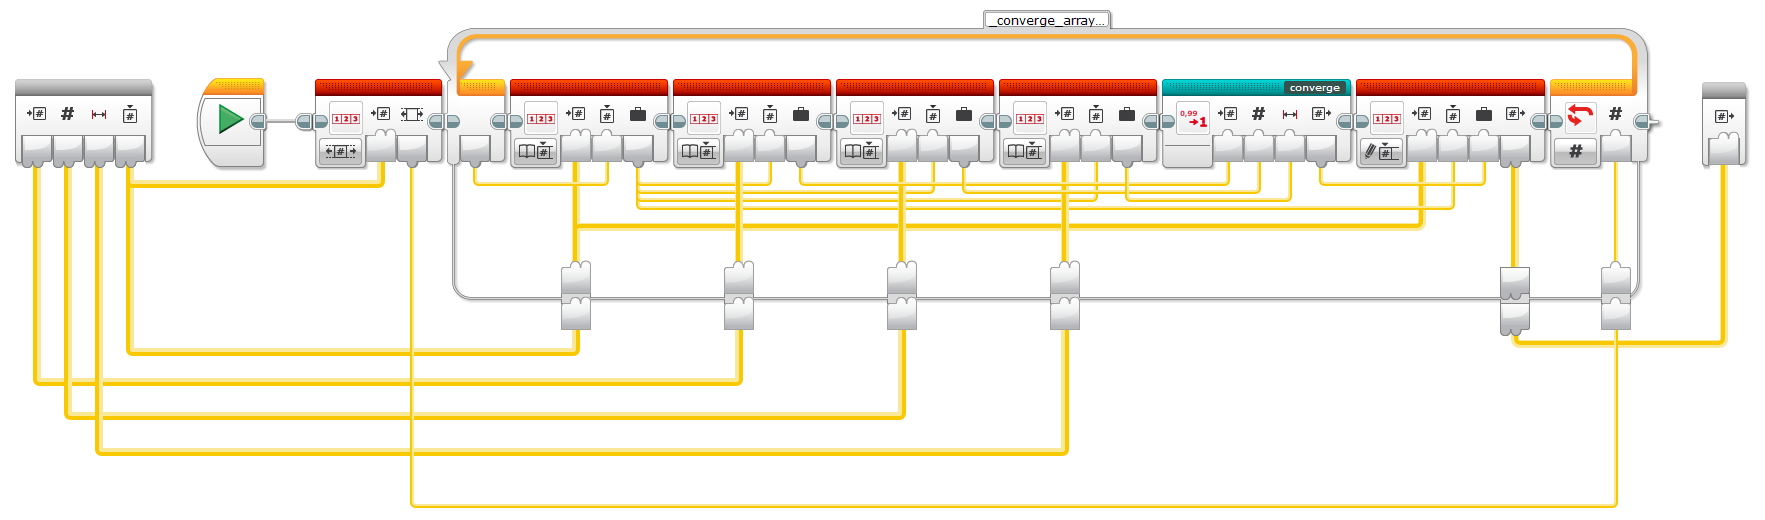
\includegraphics[width=\textwidth]{images/lego-soft/lego-soft_legolib_converge_array.png}
	\caption{Ukázka debugování za běhu programu}
	\label{fig:lego-soft_live-debuging_line-advance}
\end{figure}
\begin{figure}[h]
	\centering
	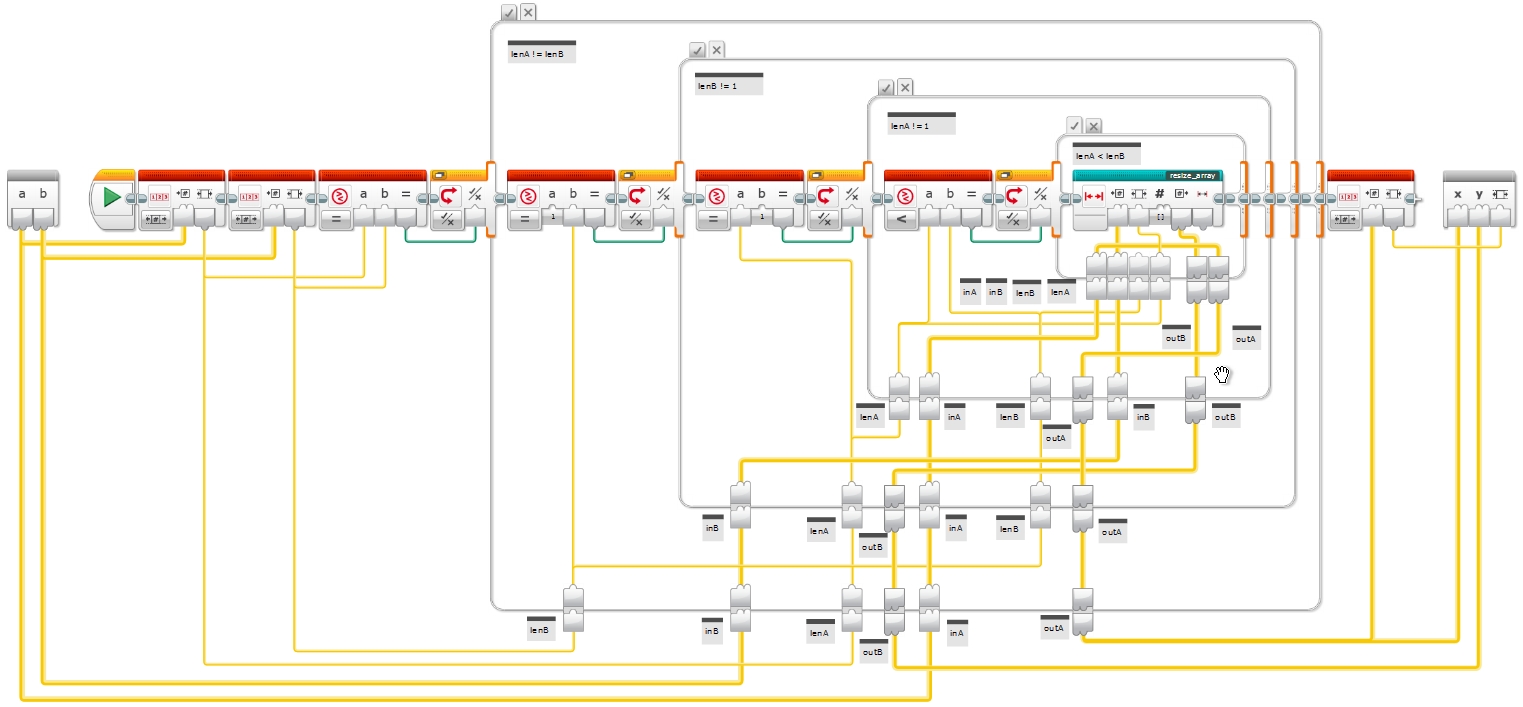
\includegraphics[width=\textwidth]{images/lego-soft/lego-soft_legolib_match_array_length.png}
	\caption{Ukázka debugování za běhu programu}
	\label{fig:lego-soft_live-debuging_line-advance}
\end{figure}



